\documentclass[12pt,oneside,a4paper]{article}

\usepackage{custom}

\newcommand{\question}
{
\addtocounter{section}{1}
\section*{Question \thesection}
}

\newcommand{\myX}[2]{x_{#1,\text{#2}}}
\newcommand{\xSemaine}[1]{\myX{s}{#1}}
\newcommand{\xn}{\xSemaine{n}}
\newcommand{\xsup}{\xSemaine{sup}}
\newcommand{\xstock}{\xSemaine{stock}}
\newcommand{\xretard}{\xSemaine{retard}}
\newcommand{\xsst}{\xSemaine{sst}}

\newcommand{\texttts}[1]{{\small\texttt{#1}}}

\title{Projet d'optimisation}
\author{Groupe 1}
\date{\today}

\begin{document}

\maketitle

\question %1

\subsection*{Variables}
Le tableau~\ref{tab:variablesQuestion1} contient les différentes variables $x_{s,\lambda}$
qui correspondent au nombre de smartphones pour chaque semaine $s$
avec la caractéristique $\lambda$.

\begin{table}[h]
  \begin{center}
  \begin{tabular}{|c|l|}
    \hline
    Variable & Caractéristiques des smartphones \\
    \hline
    \hline
    $\xn$ & Produits au \emph{salaire normal}. \\
    \hline
    $\xsup$ & Produits pendant les \emph{heures supplémentaires}. \\
    \hline
    $\xstock$ & Conservés en \emph{stock}. \\
    \hline
    $\xretard$ & Vendus une semaine en \emph{retard}. \\
    \hline
    $\xsst$ & Sous-traités. \\
    \hline
  \end{tabular}
  \caption{Variables de la modélisation de la ligne d'assemblage.}
  \label{tab:variablesQuestion1}
  \end{center}
\end{table}

\subsection*{Contraintes}
Voici les contraintes du problème de la planification 
de la ligne d’assemblage à personnel constant.
On pose que $\Delta x_{s,\lambda} = x_{s,\lambda} - x_{s-1,\lambda}$.
\begin{align*}
  \Delta\xstock + \texttts{demande}(s) &= \xn + \xsup 
  + \xretard + \xsst - \myX{s-1}{retard} &\forall s \\
  \myX{s-1}{retard} + \Delta\xstock &\leq \xn + \xsup + \xsst &\forall s \\
  \myX{0}{stock} &= \texttts{stock-initial} \\
  \myX{T}{stock} &= \texttts{stock-initial} \\
  \myX{T}{retard}&= 0 \\
  \xn &\leq 35\cdot \texttts{nb\_ouvriers}/ d_{a,h}
  &\forall s \\
  \xsup &\leq \texttts{nb\_max\_heure\_sup}\cdot\texttts{nb\_ouvriers}/ d_{a,h}
  &\forall s \\
  \xsst &\leq \texttts{nb\_max\_sous\_traitant} &\forall s \\
  x_s &\geq 0 &\forall s
\end{align*}

\subsection*{Fonction objectif}
\[
  \mbox{minimiser } 
  \sum_{s=1}^{T} 
  c_m\, \xn + (c_m + d_{a,h} \, c_{hs})\, \xsup
  + c_s\, \xstock + c_r\, \xretard + c_{sst}\, \xsst
\]
Le tableau~\ref{tab:constantesQuestion1} contient les abréviations
des constantes utilisées.
\begin{table}[h]
  \begin{center}
  \begin{tabular}{|c|l|}
    \hline
    Paramètre & Constante représentée \\
    \hline
    \hline
    $c_m$ & \texttt{cout\_materiaux} \\
    \hline
    $c_{hs}$ & \texttt{cout\_heure\_sup} \\
    \hline
    $c_s$ & \texttt{cout\_stockage} \\
    \hline
    $c_r$ & \texttt{cout\_retard} \\
    \hline
    $c_{sst}$ & \texttt{cout\_sous\_traitant} \\
    \hline
    $d_{a,h}$ & \texttt{duree\_assemblage}/60 \\
    \hline
  \end{tabular}
  \caption{Constantes de la modélisation de la ligne d'assemblage.}
  \label{tab:constantesQuestion1}
  \end{center}
\end{table}

A ce stade, le fait de ne pas imposer l'intégralité des variables
parait problèmatique dans le sens où les solutions ne sont pas 
garanties d'être entières. Ce qui n'est pas envisageable 
vu que celles-ci représentent des quantités de smartphones.
Par exemple, 
$\xn$ ne sera probablement pas entier si $1/d_{a,h}$ ne l'est pas.
% TODO autre mot que problablement ? "il est possible que" 

\question %2

Il est possible de garantir que notre modèle linéaire continu
admette toujours une solution entière sous certaines hypothèses.
Une première hypothèse est que tous les éléments du 
vecteur \texttt{demande} soient entiers.
Il faut également que les constantes \texttt{stock-initial},
\texttt{nb\_max\_heure\_sup}, \texttt{nb\_max\_sous\_traitant},
\texttt{nb\_ouvriers} et $1/d_{a,h}$ soient entières.
% TODO nécéssaire de spécifier même celles qui parraissent évidente? 

\subsubsection*{Preuve}
Pour le prouver, nous allons reformuler notre problème sous la forme d'un problème de flot de coût minimum.
Soit le graphe orienté G(V,E), où V représente l'ensemble des noeuds et E l'ensemble des arrêtes.
Il est utile à ce stade de s'aider d'un schéma représentant le graphe. 
Celui-ci est repris à la figure \ref{fig:schema_flot}.
V compte un noeud pour chauqe semaine et un noeud initial.
On a donc $V := {0, 1, 2, ..., T}$ où 0 est le noeud initial et s est le noeud de la semaine s.
Définissons maintenant les arrêtes de notre graphe.
Pour le noeud 0, on définit $$V^{-}(0) = \{s_1, s_2, s_3 \, \forall s \ne 0\}$$ avec $$\{(0, s_1), (0, s_2), (0, s_3)\} \in E \, \forall s$$
$s_1, s_2, s_3$ représentent les différentes manières de produire les smartphones, c'est-à-dire les ouvriers au salaire normal, les ouvriers au salaire des heures supplémentaires et la sous-traitance.
Il y a donc trois arcs entre les noeuds 0 et s.
Pour le noeud initial,  $$V^{+}(0) = \emptyset$$
Définissons ensuite les arrêtes des noeuds corrspondnats aux semaines \\
$$V^{-}(s) = \{s+1 \, \forall s \ne 0\}$$ avec $$\{(s, s+1)\} \in E \, \forall s \ne 0, T$$
Et, $$V^{+}(s) = s-1 \, \forall s \ne 0\}$$ avec $$\{(s, s-1)\} \in E \, \forall s \ne 0, 1$$
Nous devons encore définir les termes sources pour chaques noeuds ainsi que les capacités maximales pour chaque arc.
Soit $$b_s = - demande(s), s \in V \backslash \{0\}$$
Et $$b_0 = \sum_{s=1}^{T} demande(s)$$
On a aussi $$b_1 = stock\_initial$$
Et $$b_T = - stock\_initial$$
Soient $h_{ij}$ avec $(i, j) \in E$ les capacités maximales dans l'arc $(i, j)$.
On a $\, \forall s \ne 0$ 
$$h_{0, s_1} = 35\cdot \texttts{nb\_ouvriers}/ d_{a,h} $$
$$h_{0, s_2} = \texttts{nb\_max\_heure\_sup}\cdot\texttts{nb\_ouvriers}/ d_{a,h} $$
$$h_{0, s_3} = \texttts{nb\_max\_sous\_traitant} $$
Le graphe maintenant défini, on peut définir le problème de minimisation suivant :
\paragraph{Variables}
Soit $x_{ij}$ le flot dans l'arc $(i, j)$.
\paragraph{Objectif}
Le coût total est minimisé.
$$\sum_{(i, j) \in E} c_{ij} x_{ij}$$
\paragraph{Equations} Le flot est conservé en chaque noeud $$\sum_{k \in V^{+}(i)} x_{ik} - \sum_{k \in V^{-}(i)} x_{ki} = b_i \, \, i \in V$$
Les capacités maximales ne sont pas dépassées $$0 \leq x_{ij} \leq h_{ij} \, \, (i, j) \in E$$
On peut maintenant utiliser le théorème suivant pour conclure que, si nos hypothèses sont vérifiées, notre problème admettra au moins une solution entière.
\paragraph{Théorème}
Si les demandes $b_i$ et les capcités $h_{ij}$ d'un problème de flot de coût minimum sont entières alors il existe une solution optimale entière.
\begin{figure}[hp]
	\centering
		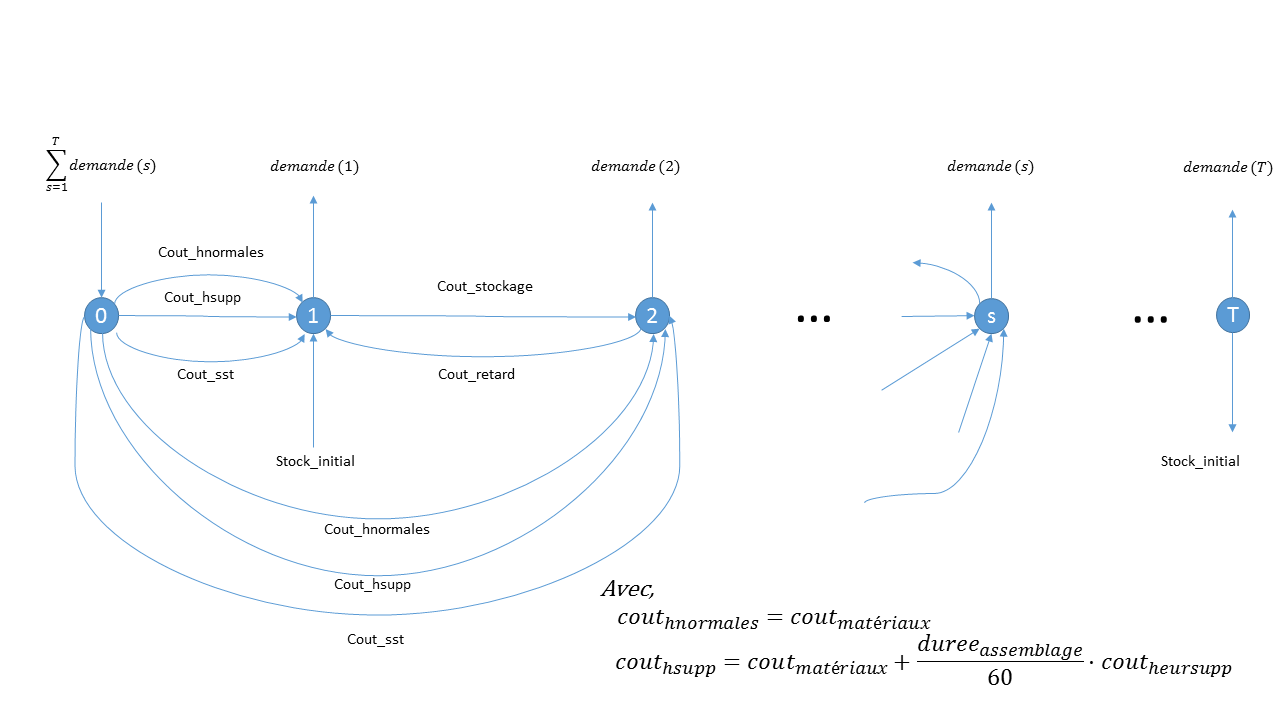
\includegraphics[scale = 0.5]{Schema_flot.png}
	\caption{Schéma représentant le graphe utilisé pour définir le problème de flot de coût minimal}
	\label{fig:schema_flot}
\end{figure}




\end{document}